\scanpage{45}
% archive sheet number: 44
\[\prod_{x\in X}\widehat{{\unsure{\mathscr O|\mathcal O}}}_x\]
\margin{{\unsure{Adèles}} pour plusieurs {\unsure{dimensions}}}
\figure{\begin{tikzpicture}\draw (0,1.5) .. controls (.1,1) and (-.1,.3) .. (0,0) -- (4,0);\end{tikzpicture}}
\[\prod_{\substack{\mathrm{local}\\x_1\in X_1}}\widehat{\mathscr O}_{x_1}\otimes_{\underline{\mathscr O}_{x_1}}K=\prod_{\mathrm{local}}K_D\]
\[\prod_{x_1}\deleted{{\unsure{\mathrm{lim}|\mathrm{loc}}}}\prod_{\substack{\mathrm{local}\\\underline{x_0}\in\bar x_1}}\mathscr O_{[x_0,x_1]}\]
\diagram{\begin{tikzcd}[ampersand replacement=\&,column sep=large]
\displaystyle\prod_{x_0x_1(x_2)}\mathscr O_{[x_0x_1x_2]}\arrow[d]\&\mathscr O_{[x_0x_2]}=\widehat{\underline{\mathscr O}}_{x_0}\otimes_{\underline{\mathscr O}_{x_0}}K\\
\mathscr O_{[x_0x_1]}\otimes_{\mathscr O_{x_1}}K\&
\end{tikzcd}}
\diagram{\begin{tikzcd}[ampersand replacement=\&,column sep=tiny,row sep=large]
K\arrow[d,equal]\&\underbrace{\longrightarrow}_{\widehat{\mathscr O}_{x_1}\otimes_{\underline{\mathscr O}_{x_1}}K}\&I_{x_1}\&\underbrace{\longrightarrow}_{\underline{\mathscr O}_{[x_0,x_1]}}\&I_{x_0}\\
\widehat{\underline{\mathscr O}}_{x_2}\&\&\widehat{\deleted{{\unsure{t|b}}}\underline{\mathscr O}}_{{\unsure{x_p|x_1}}}\&\&\widehat{\underline{\mathscr O}}_{x_0}
\end{tikzcd}}
\figure{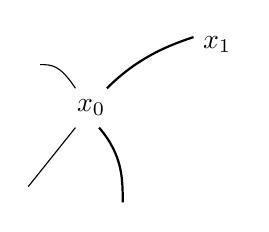
\begin{tikzpicture}
\node at (0,0) {$x_0$};\node at (1.6,.8) {$x_1$};
\draw[thick] (.2,.25) .. controls (.6,.65) and (1,.8) .. (1.3,.9);
\draw (-.2,.25) .. controls (-.4,.55) and (-.5,.55) .. (-.65,.55);
\draw (-.2,-.25) -- (-.8,-1);
\draw[thick] (.1,-.25) .. controls (.4,-.6) and (.4,-.9) .. (.4,-1.2);
\end{tikzpicture}}
\[\begin{array}{ccc}\widehat{\underline{\mathscr O}}_{x_0}&\widehat{\mathscr O}_{x_1}&\widehat{\mathscr O}_{x_2}\\{\unsure{m_0|\mathfrak m_0}}&m_1&m_2\end{array}\]
\[\prod_{x\in X}\mathscr O_{[x]}\]
\[\prod_{\substack{\mathrm{local}\\x_1\in X_1}}\mathscr O_{[x_1,x_2]}\qquad{\unsure{\mathscr O.}}\]
\[\prod_{x_1}\prod_{\substack{\mathrm{local}\\x_0}}\mathscr O_{[x_0,x_1]}\]
\figure{\begin{tikzpicture}\draw (0,0)--(.5,1.8);\end{tikzpicture}}
\diagram{\begin{tikzcd}[ampersand replacement=\&,column sep=small,row sep=large]
\displaystyle\prod_{\underline{x_0}}\mathscr O_{[x_0]}\arrow[d,"\text{{\unsure{localisat|localisant}}}"]\&\&\\
\displaystyle\prod_{\underline{x_1}}\prod_{\substack{\mathrm{local}\\\underline{x_0}}}\mathscr O_{[x_0,x_1]}\arrow[d,"\overline{\text{{\unsure{localisat|localisant}}}}"]\&\displaystyle\prod_{\underline{x_1}}\mathscr O_{[\bar x_1]}\arrow[l]\arrow[d,"\text{{\unsure{localisant|localisat}}}"]\&\\
\displaystyle\prod_{\substack{{\unsure{\mathrm{rest.}|\mathrm{restr.}}}\\\underline{x_0}}}\prod_{\substack{\mathrm{rest.}\\\underline{x_1}}}\mathscr O_{[x_0,x_1,x_2]}\&\displaystyle\prod_{\substack{\mathrm{local}\\(\underline{\underline{x_1}},x_2)}}\mathscr O_{[\bar x_1x_2]}\arrow[l]\&\displaystyle\prod_{x_2}\mathscr O_{[x_2]}=K\arrow[l]
\end{tikzcd}}
\[\underline{\mathscr O}_{[\underline{\underline{x_1}},x_2]}\qquad\deleted{\prod_{x_1}}\]
\[\deleted{{\unsure{\mathscr A|\mathcal A}}_{i_0--i_{p-1}}}\qquad\deleted{{\unsure{\sum x_1|\prod}}_{x_1}}\]
\figure{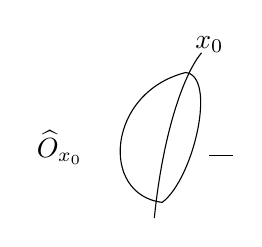
\begin{tikzpicture}
\node at (-1.3,-.3) {$\widehat{\mathscr O}_{x_0}$};\node at (.6,1) {$x_0$};
\draw (0,-1) .. controls (-.8,-.9) and (-.7,.4) .. (.3,.65) .. controls (.7,.6) and (.4,-.7) .. (0,-1);
\draw (-.1,-1.2) .. controls (0,-.2) and (.25,.6) .. (.5,.9);
\draw (.6,-.4)--(.9,-.4);
\end{tikzpicture}}
\diagram{\begin{tikzcd}[ampersand replacement=\&,row sep=small]
\mathscr O_{[x_0x_1]}\arrow[d]\\
\displaystyle\prod_{x_0x_1}\mathscr O_{[x_0x_1x_2]}
\end{tikzcd}}
\[\mathscr A_{i_0--i_p}\qquad\mathscr A_{i_1\cdots i_{p-1}}\]
\deleted{{\unsure{localisé|localis.}}}
\[x_{i_0}\quad x_{i_1}-x_{i_p}\]
\[i_0<i_1<\cdots<i_p\]
\[-\]
